\section{Contexte}

Dans \gls{lc3d}, la scène virtuelle est géré grâce à Opengl\todo{ref!}, une \gls{librarie} graphique.
Pour mieux comprendre certains termes qui seront abbordé par la suite, voici quelques notion de base sur OpenGL :

Les différents objets virtuelles sont représenté par un ensemble de point 3D appelé “sommet”.
Un sommet est positionné dans l’espace virtuelle à partir d’un repère 3D qui est représenté par un sommet (dit l’origine du repère) et trois vecteur unitaire, caractérisé par un sommet de départ (l’origine), une direction et une longueur (dit la “norme”) qui constituera l’unité de base dans la scène (Figure ~\ref{fig:repere}).

Les trois vecteur sont représentatif des axes X , Y et Z,  pour faire simple, on peut dire dans notre cas que l’axe X est relatif à la gauche ou à la droite, l’axe Y au fait d’etre avancé ou éloigné et l’axe Z au haut ou au bas. Cela est schématisé comme suit : 

\begin{figure}[!ht]
\centering
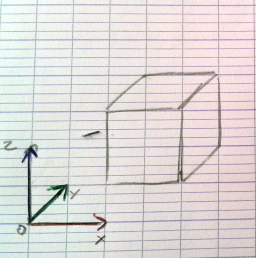
\includegraphics[width = 4cm] {images/croquisRepere3d.jpg} 
\caption{Représentation d'un objet 3D virtuelle par rapport au repère 3D}
\label{fig:repere}
\end{figure}

Ainsi si on choisit de déplacer l’ensemble des sommets caractérisant notre objet dans la direction du vecteur (OX), notre objet se retrouve alors décalé vers la droite.

\begin{figure}[!ht]
\centering
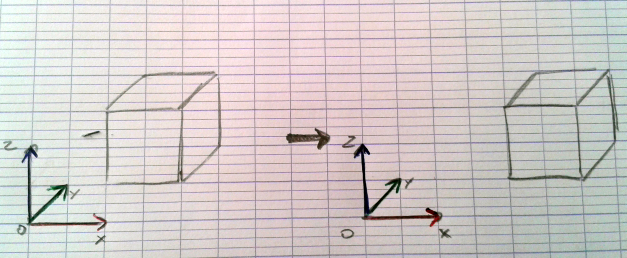
\includegraphics[width = 8cm] {images/croquisTranslation.jpg}
\caption{translation}
\label{fig:transformation}
\end{figure}

le déplacement illustré dans la figure \ref{fig:transformation} est appelé une transformation. Les transformations principales nous permettront de déplacer nos objets d’une position à une autres en suivant une direction (translation), de changer leur orientation (rotation), ou encore d’effectuer un changement d’échelle (agrandir ou rétrécir).

Ces transformations sont réalisés grâce à ce qu’on appelle une matrice, qui peut être vu comme un tableau de valeurs numériques (dans notre cas un tableau de 4 colonne et 4 ligne, donc 16 valeurs). La transformation s’effectue par un calcul mathématiques entre le sommet et la matrice.

La matrice responsable des transformations appliqué aux objets virtuelle et qui nous permet ainsi de situer nos objets par rapport au repère 3D est appelé matrice de modèle mais ce n’est pas la seule à intervenir.

En effet dans notre monde virtuelle nous avons aussi ce qu’on appelle une caméra qui va correspondre au point de vue de l’utilisateur. Elle est représenté par trois vecteurs caractéristiques :
le vecteur “eye” qui indique la position de la caméra dans le monde virtuel, 
le vecteur “target” qui indique la direction à laquelle on regarde
le vecteur “up” qui indique ou se situe le haut
Ainsi si l’on souhaite voir un objet sous différents angles ou se déplacer dans la scène c’est cette camera qu’on bougera, la matrice de transformation associé est appelé la matrice de vue.

\begin{figure}[!ht]
\centering
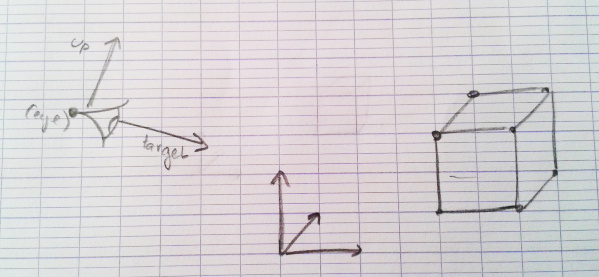
\includegraphics[width = 8cm] {images/croquisVue.jpg}
\caption{Représentation de la camera dans la scène virtuelle}
\label{fig:vue}
\end{figure}

Dans la version d’OpenGL utilisé dans \gls{lc3d} (version 2) on utilise qu’une seule matrice, la matrice ModelView qui est la combinaison de la matrice du Modèle et de la matrice de vue.


A cela s’ajoute encore une autre matrice, la matrice de projection, qui elle sera responsable de notre champ de vision et de la perspective de la scène visualisé. Cela se manifeste entre autre par la capacité à distinguer un objet proche d’un objet éloigné, en appliquant une transformation qui comme notre perception du monde réel, nous fera apparaître les objets proche plus gros et les objets éloigné plus petit.

\begin{figure}[!ht]
\centering

\includegraphics[width = 2cm] {images/nop.png}
\caption{Illustration du resultat obtenu avec une matrice de projection}
\label{fig:projection}
\end{figure}

%En clair, ce sont deux matrice , la matrice de projection, et la matrice de modelview qui sont responsable de la bonne visualisation du rendu de notre scène virtuelle.

%De ce fait, dans le cadre de la realité augmenté, pour assurer la cohérence entre la scène réelle et virtuelle se sont ses deux matrices qu’on l’on essaye de déterminer dans \gls{lc3d}.

%Pour ce faire on effectue ce qu’on appelle une \gls{calibration}


%Dans LogyConcept3D, la détéction du sol et le respect des mesures sont lié et sont réalisé grâce à un processus appelé "\gls{calibration}".
%la calibration de l'appareil chargé de capturé l'image réelle (appareil photo, camera...), consiste à récupérer les paramètre intrèseque et extreseque de l'appareil. C'est paramètre vont nous permettre de calculé la "pose" de la caméra, c'est-à-dire de retrouver les transformation qu'un point dans l'espace subit pour être projeter sur l'image.

Maintenant dans la cadre de la réalité augmenté, pour faire la superposition avec une image réel , nous utilisons l’image en tant qu’image de fond. Ne ne considérons pas cette image comme un élément virtuelle, c’est-à-dire que quelque soit la valeur de notre matrice ModelView ou de notre matrice Projection, la visualisation de l’image reste inchangé.

On peut voir en figure \ref{fig:schemaRV1} ce que l’on obtient désormais dans notre scène virtuelle.

\begin{figure}[!ht]
\centering
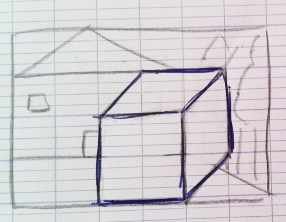
\includegraphics[width = 5cm] {images/croquisRAModelViewBefore.jpg}
\caption{Superposition d'une scène virtuelle sur une image réelle sans traitement préalable}
\label{fig:schemaRV1}
\end{figure}

Comme nous pouvons le constaté notre scène virtuelle superposé n’est pas du tout cohérente avec la scène réelle. Cependant comme vue plus haut, en modifiant la position de la caméra (matrice ModelView) et la matrice de Projection, nous pouvons modifié la visualisation de notre scène virtuelle et obtenir un resultat adéquat (Figure \ref{fig:schemaRV2}.

\begin{figure}[!ht]
\centering
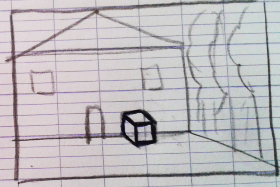
\includegraphics[width = 5cm] {images/croquisRAModelViewAfter.jpg}
\caption{Superposition d'une scène virtuelle après determination de la matrice ModelView et la matrice Projection}
\label{fig:schemaRV2}
\end{figure}

Assurer cette cohésion entre la scène réelle et la scène virtuelle fait partie des grandes problèmatiques de la réalité augmentée. Trouver les matrices ModelView et Projection adéquatent sont réalisé dans \gls{lc3d} grâce à un processus appelé "\gls{calibration}".

la calibration de l'appareil chargé de capturé l'image réelle (appareil photo, camera...), consiste à récupérer des paramètre spécifique de la caméra (paramètre intrésèque et extrinsèque). Ces paramètre nous permettront de retrouver les transformations que subit un point dans l’espace (point 3D) afin d’être projeté sur l’image résultat en 2D (pixel) . Autrement dit, cela revient à calculer ce qu’on appelle la “pose” de la caméra, c’est-à-dire la position de la caméra dans l’espace qui nous permettra pour un point 3D donné de le visualiser sur le pixel en 2D correspondant sur l’image réelle, c’est de là qu’on en déduit notre matrice de Projection et de ModelView. 

Dans \gls{lc3d} les points 3D , au nombre de 4 pour former un quadrilatère, sont défini à partir d’un objet de référence sur l’image réelle, appelé “la mire”. La mire peut être de deux type, soit un objet posé sur le sol, soit une fenêtre. C’est également à cette étape qu’on en profite pour détecter le sol,en spécifiant que la coordonnée  Z de nos points 3D est égale à 0. La longueur entre deux sommet doit également être spécifier, ce qui nous permet d’avoir le respect des mesures. Les pixels correspondant sont quand à eu, sélectionner par l’utilisateur par clique sur l’image réelle. Après cela nous pouvons créer notre scène virtuelle (Annexe création d’un projet avec LogyConcept3D Pool).

En ce qui concerne les occlusions, elle ne sont pas déduites automatiquement et doivent être masqué à la main grâce à une fonctionnalité du logiciel.
Les ombres sont quand à alle afficher automatiquement en fonction de la position du soleil. 

Même si nous obtenons un résultats correcte, le processus de calibration utilisé soulève quelques contraintes et peut être amélioré, on aboutit ainsi au sujet de mon stage
